
\begin{frame}{deliberate sharing: retrieving information}
    \begin{itemize}
    \item what about retrieving information from JavaScript?
    \item example: Google Translator API
    \item example: Token to Username API
    \vspace{.5cm}
    \item explicit mechanism for server opt-in to cross-origin requests (where webpage can read result)
        \begin{itemize}
        \item Cross-Origin Resource Sharing
        \end{itemize}
    \item \myemph{no opt-in? JS fails} like before
    \item always sends Origin --- no pretending to be innocent user
    \end{itemize}
\end{frame}


\begin{frame}{cross-origin resource sharing}
    \begin{itemize}
    \item sometimes want exceptions to usual origin policy:
    \vspace{.5cm}
    \item let scripts on foo.com load data from bar.com
        \begin{itemize}
        \item example: bar.com running maps API
        \end{itemize}
    \item need mechanism for bar.com to give permission
        \begin{itemize}
        \item don't accidentally leak logged-in only info
        \end{itemize}
    \item historically didn't worry about this:
        \begin{itemize}
        \item no restrictions on loading images/scripts from elsewhere
        \item \ldots even though they may be based on cookies/etc.
        \end{itemize}
    \end{itemize}
\end{frame}

\begin{frame}{Fetch standard}
    \begin{itemize}
    \item modern browsers: Fetch standard
        \begin{itemize}
        \item {\scriptsize\url{https://fetch.spec.whatwg.org/}}
        \end{itemize}
    \item defines procedures for fetching resources in general
        \begin{itemize}
        \item loading imgs, scripts
        \item requests from JavaScript
        \end{itemize}
    \end{itemize}
\end{frame}

\begin{frame}{Fetch request types}
    \begin{itemize}
    \item standard defines request types with different rules:
    \item navigate --- go to whole new web page
    \item no-cors --- `old' default
        \begin{itemize}
        \item limit to `normal' methods
        \item very limited setting of HTTP headers by scripts
        \item \myemph<2>{response contents not directly visible to scripts} (but could, e.g., be displayed as image, set image size, etc.)
        \end{itemize}
    \item cors
        \begin{itemize}
        \item remote server needs to specify what's allowed
        \end{itemize}
    \item same-origin
        \begin{itemize}
        \item remote server needs to have same origin
        \end{itemize}
    \end{itemize}
\end{frame}

\begin{frame}[fragile]{crossorigin attribute}
    \begin{itemize}
    \item \verb|<img src=...>| --- no-cors
    \item \verb|<img src=... crossorigin=anonymous>| --- cors, don't send cookies
    \item \verb|<img src=... crossorigin=use-credentials>| --- cors, do send cookies
    \end{itemize}
\end{frame}

% FIXME: CORS preflighting

\begin{frame}{preflighting}
    \begin{itemize}
    \item want server to tell us whether request is allowed
    \item problem: normally server only responds after making request anyways
    \vspace{.5cm}
    \item solution: make `preflight' request to ask
    \end{itemize}
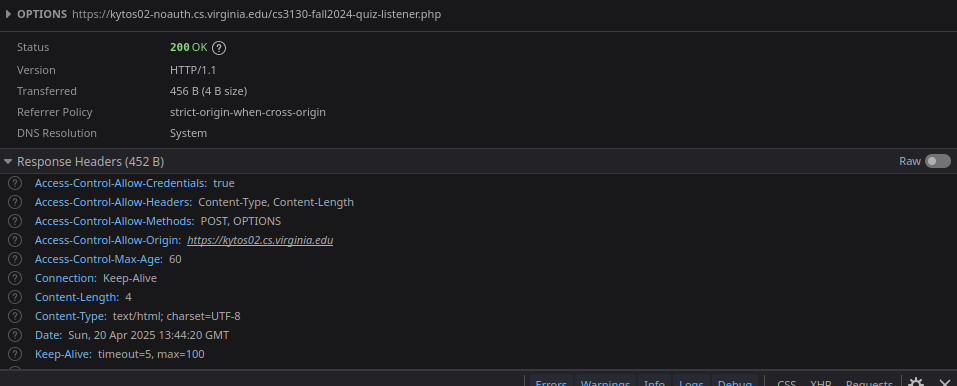
\includegraphics[height=0.5\textheight]{../web/cors-preflight-ex}
\end{frame}

\begin{frame}{Access-Control-Allow\ldots}
    \begin{itemize}
    \item Origin --- who can make requests
    \item Headers --- what headers scripts can read
    \item Credentials --- should request include cookies/other auth. info
        \begin{itemize}
        \item NOTE: not even checked on no-CORS request!
        \item NOTE: client may not include cookies for privacy reasons, still
        \item NOTE: script making request can ask to not include cookie
        \end{itemize}
    \item Request-Headers --- request headers scripts can set
    \item Request-Method
    \item Max-Age --- how long to remember these settings before asking again
    \end{itemize}
\end{frame}


\begin{frame}{Cross-Origin-*-Policy}
    
\end{frame}

